\documentclass[border=3mm,tikz,preview]{standalone}
\usetikzlibrary{intersections}
\usetikzlibrary{positioning}
\usetikzlibrary{shapes.misc}

\tikzset{cross/.style={cross out, draw=black, minimum size=2*(#1-\pgflinewidth), inner sep=0pt, outer sep=0pt},
	%default radius will be 1pt. 
	cross/.default={2pt}}

\begin{document}
	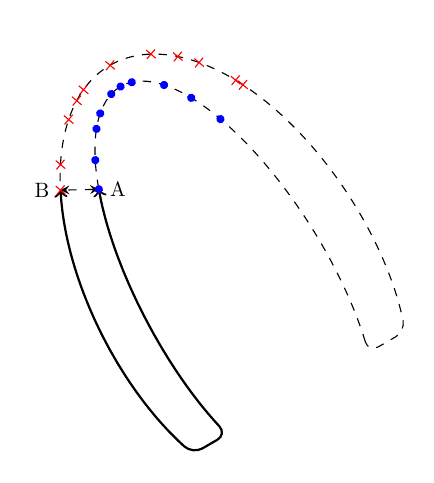
\begin{tikzpicture}
		\begin{scope}[rotate=30]
%			\draw[step=0.5,help lines,black!20] (-5, -5) grid (5, 5);
			\draw[thin, dashed, rounded corners] (0,0) 
			arc[x radius=12mm, y radius=30mm, start angle=-30, end angle=210]
			coordinate[pos=0.3] (A1)
			coordinate[pos=0.35] (A2)
			coordinate[pos=0.4] (A3)
			coordinate[pos=0.47] (A4)
			coordinate[pos=0.5] (A5)
			coordinate[pos=0.53] (A6)
			coordinate[pos=0.58] (A7)
			coordinate[pos=0.61] (A8)
			coordinate[pos=0.66] (A9)
			coordinate[pos=0.7] (A10)
			coordinate[pos=1] (A11)
			-- ++ (-0.5,0)
			arc[x radius=18mm, y radius=32mm, start angle=210, end angle=-30]
			coordinate[pos=0.3] (B1)
			coordinate[pos=0.33] (B2)
			coordinate[pos=0.39] (B3)
			coordinate[pos=0.42] (B4)
			coordinate[pos=0.44] (B5)
			coordinate[pos=0.5] (B6)
			coordinate[pos=0.57] (B7)
			coordinate[pos=0.61] (B8)
			coordinate[pos=0.64] (B9)
			coordinate[pos=0.69] (B10)
			coordinate[pos=0.7] (B11)
			-- cycle;
				\fill[blue] (A1) circle (1.5pt);
				\fill[blue] (A2) circle (1.5pt);
				\fill[blue] (A3) circle (1.5pt);
				\fill[blue] (A4) circle (1.5pt);
				\fill[blue] (A5) circle (1.5pt);
				\fill[blue] (A6) circle (1.5pt);
				\fill[blue] (A7) circle (1.5pt);
				\fill[blue] (A8) circle (1.5pt);
				\fill[blue] (A9) circle (1.5pt);

				\node [right=0.05cm of A10, scale=0.75] {A};
				\node [left=0.05cm of B1, scale=0.75] {B};

				\fill (B2) node[cross,rotate=5, red] {};
				\fill (B3) node[cross,rotate=5, red] {};
				\fill (B4) node[cross,rotate=5, red] {};
				\fill (B5) node[cross,rotate=5, red] {};
				\fill (B6) node[cross,rotate=5, red] {};
				\fill (B7) node[cross,rotate=5, red] {};
				\fill (B8) node[cross,rotate=5, red] {};
				\fill (B9) node[cross,rotate=5, red] {};
				\fill (B10) node[cross,rotate=5, red] {};
				\fill (B11) node[cross,rotate=5, red] {};
				\draw[stealth-stealth, dashed] (A10) -- (B1);
				\draw[rounded corners, <->, thick] (A10) arc[x radius=12mm, y radius=30mm, start angle=138, end angle=210] 
				-- ++ (-0.5,0)
				arc[x radius=18mm, y radius=32mm, start angle=210, end angle=138];
								\fill[blue] (A10) circle (1.5pt);
												\fill (B1) node[cross,rotate=5, red] {};
%			\draw[thin, red] (1,0) 
%			arc[x radius=12mm, y radius=24mm, start angle=-30, end angle=210]
%			-- ++ (-0.5,0)
%			arc[x radius=18mm, y radius=32mm, start angle=210, end angle=-30]
%			-- cycle;
%			\draw[red] (0,4.25) circle (5);
%			\fill[red] (0,4.25) circle (2mm);
		\end{scope}
%		\begin{scope}[xshift=110mm,rotate=210]
%			\draw[very thick,fill=gray] (1,2)
%			arc[x radius=12mm, y radius=24mm, start angle=-30, end angle=210]
%			-- ++ (-0.5,0)
%			arc[x radius=18mm, y radius=32mm, start angle=210, end angle=-30]
%			-- cycle;
%			\draw[red] (0,4.25) circle (5);
%			\fill[red] (0,4.25) circle (2mm);
%		\end{scope}
%		\begin{scope}[shift={(205mm,-20mm)},rotate=210,scale=0.5]
%			\draw[very thick,fill=gray] (1,0)
%			arc[x radius=12mm, y radius=24mm, start angle=-30, end angle=210]
%			-- ++ (-0.5,0)
%			arc[x radius=18mm, y radius=32mm, start angle=210, end angle=-30]
%			-- cycle;
%			\draw[red] (0,4.25) circle (5);
%			\fill[red] (0,4.25) circle (2mm);
%		\end{scope}
	\end{tikzpicture}
\end{document}